%%%%%%%%%%%%%%%%%%%%%%%%%%%%%%%%%%%%%%%%%%%%%%%%%%%%%%%%%%%%%%%%%%%%%%%%%%%

\documentclass{standalone}

\usepackage{amsmath}
\usepackage{mathptmx}
\usepackage{pgfplots}
\usetikzlibrary{external}
\tikzexternalize{bacteria}
\pgfplotsset{compat=1.15}

%% IEEE uses Times Roman font, so we'll default to Times.
%% These three commands make up the entire times.sty package.
\renewcommand{\rmdefault}{ptm}
\renewcommand{\ttdefault}{pcr}
\normalfont\selectfont

\begin{document}

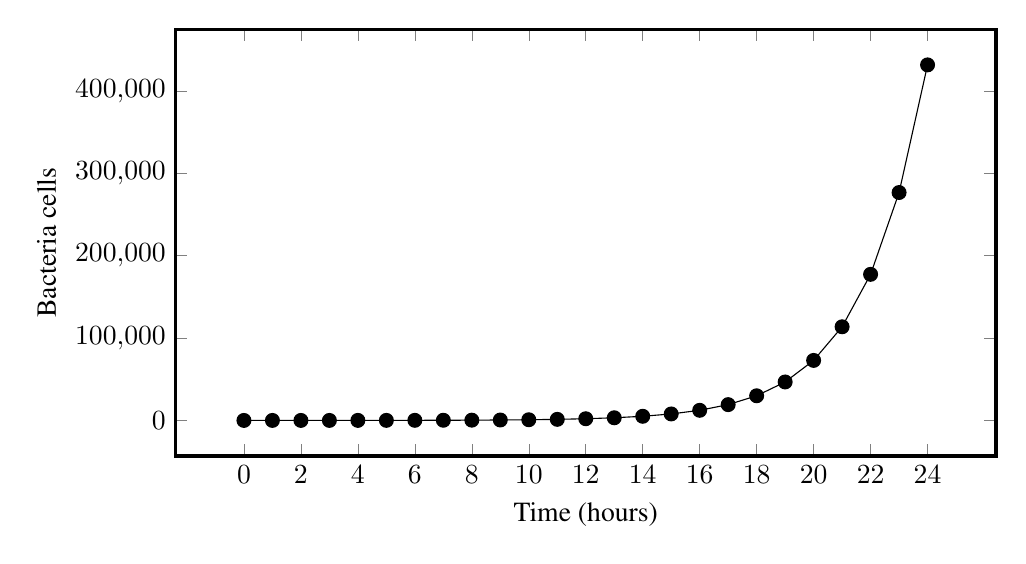
\begin{tikzpicture}
\tikzset{%%
  every mark/.append style={scale=1.0},%%
  scale=1.0%%
}
\pgfplotsset{%%
  every axis/.append style={font=\normalsize}%%
}
%%
\begin{axis}[%%
  axis line style=very thick,%%
  dotStyle/.style={mark size=2.5,black,mark color=black,mark=*},%%
  enlargelimits=true,%%
  height=7cm,%%
  plotStyle/.style={%%
    domain=4:17,%%
    mark=none,%%
    smooth,%%
    thick%%
  },%%
  width=12cm,%%
  %% x axis
  xlabel={\normalsize Time~(hours)},%%
  xtick={0,2,4,6,8,10,12,14,16,18,20,22,24},%%
  xticklabels={$0$,$2$,$4$,$6$,$8$,$10$,$12$,$14$,$16$,$18$,$20$,$22$,$24$},%%
  %% y axis
  ylabel={\normalsize Bacteria cells},%%
  scaled y ticks=false,%%
  y tick label style=/pgf/number format/fixed%%
]
%%
%%
\addplot[dotStyle] coordinates {
  (0,10.000000)
  (1,15.600000)
  (2,24.336000)
  (3,37.964160)
  (4,59.224090)
  (5,92.389580)
  (6,144.127744)
  (7,224.839281)
  (8,350.749279)
  (9,547.168875)
  (10,853.583445)
  (11,1331.590174)
  (12,2077.280672)
  (13,3240.557848)
  (14,5055.270243)
  (15,7886.221580)
  (16,12302.505665)
  (17,19191.908837)
  (18,29939.377785)
  (19,46705.429345)
  (20,72860.469778)
  (21,113662.332854)
  (22,177313.239252)
  (23,276608.653233)
  (24,431509.499043)
};
\end{axis}
\end{tikzpicture}

\end{document}
